\chapter{Introduction}

The rising popularity of video games has transformed them from niche entertainment into a mainstream medium. As a result, game development has attracted a diverse audience, including enthusiasts with limited programming experience. To meet the growing demand for accessible game development tools, various frameworks and platforms have been developed. These tools aim to simplify the creation process, enabling developers to bring their visions to life without requiring extensive coding expertise.

One genre that holds a special place in gaming history is point-and-click adventure, which emerged in the early 1980s and continues to influence the industry to this day. Despite its seemingly straightforward gameplay, creating a point-and-click adventure game involves implementing complex systems, such as a walking system, inventory mechanics, dialogue trees, and puzzle design. For novice developers, replicating these systems can be a significant hurdle.

The goal of this Bachelor thesis is to design and implement a framework in the Unity game engine tailored to the development of 2D point-and-click adventure games. This framework will prioritize functionality, user-friendliness, and accessibility, empowering beginner to intermediate game developers to create engaging games without requiring advanced programming knowledge. The framework will also allow for the rapid prototyping of game ideas, facilitating experimentation and creativity.

By addressing the unique challenges associated with point-and-click adventure game development, this thesis seeks to provide a valuable tool for aspiring developers, encouraging innovation within this beloved genre.

\section{Point-and-click adventure games}
\subsection{Definition}


\subsection{History}
The emergence of point-and-click adventure games can be traced back to the 1960s, although determining the exact origins of the genre is challenging. Early text-based adventures like \textit{The Sumerian Game} (1964) introduced simple verb-noun parsers that allowed players to interact with the game world by typing commands. \cite{Salter2014}[p. 29].  Building on this foundation, two notable predecessors to the point-and-click genre, \textit{Colossal Cave Adventure} (1976) and \textit{Mystery House} (1980), took the first steps toward integrating graphics into adventure gameplay. These games, while still reliant on text-based commands, incorporated static visuals to represent the game world, marking a significant departure from the purely text-driven interfaces of earlier adventure titles. The next stage of evolution introduced animated visuals and greater graphical complexity, allowing players to manipulate an avatar directly. For instance, in games influenced by \textit{Mystery House}, such as \textit{Valhalla} (1983), players could input commands like “go west” to move their avatar within the graphical environment \cite{Salter2014}[p. 38]. 

These developments paved the way for a radical shift in interaction methods, as the incorporation of mouse technology transformed gameplay. Screens became clickable, enabling players to point to places or objects in the graphics to interact with them, replacing typed commands with more intuitive and immediate actions.


\begin{figure}
\centering
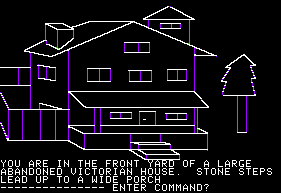
\includegraphics{img/Mystery_House.png}
\caption{The opening scene from Myster House (1980). Source: https://commons.wikimedia.org\cite{wiki:MysteryHouse}}
\label{fig:g}
\end{figure}
\todo{picture is completely off!}

This is where the contenders for the title of the first point-and-click adventure game come into the scene, among those being \textit{Enchanted Scepters}. For many years, this game was thought to have debuted in 1984. However, subsequent investigations revealed that its release likely occurred later, in November 1985. This revelation has shifted the discussion, with \textit{Deja Vu: A Nightmare Begins}, released at least a month earlier, now emerges as a leading candidate for the first true point-and-click adventure game \cite{Pfenning2024}.

The ambiguity surrounding these early releases reflects the gradual evolution of the genre, as developers experimented with interactive storytelling and gameplay mechanics. These pioneering efforts laid the groundwork for the point-and-click adventure games that followed, shaping the genre into the recognizable form that captivated audiences in the years to come.

Point-and-click adventure games experienced their golden age in the late 1980s and early 1990s, with iconic titles such as \textit{The Secret of Monkey Island} (1990), \textit{Beneath a Steel Sky} (1994), and \textit{Myst} (1994) captivating players with their innovative storytelling and puzzle-solving gameplay. However, as the decade progressed, the popularity of the genre waned\cite{Qaffas202022}, with fewer mainstream releases and a shift to niche titles such as the \textit{Nancy Drew} game series.

In recent years, the point-and-click adventure genre has undergone a renaissance. Modern titles such as \textit{Thimbleweed Park} (2017) and \textit{Return to Monkey Island} (2022) have revived interest by paying homage to the retro roots of the genre while incorporating modern design elements. This resurgence has also been fueled by the cinematic storytelling approach pioneered by \textit{Telltale Games}, whose narrative-driven series brought the genre back into the mainstream spotlight.

The renewed interest in point-and-click adventure games highlights their timeless appeal and presents an opportunity for new developers to explore the genre. Building on its rich legacy, aspiring game creators can reimagine and modernize these games for contemporary audiences. This cultural revival underscores the need for accessible development tools to support and sustain the creative evolution of this genre.